\section{モデル実行方法の概要}
%====================================================================================

SCALE-LESモデルの実行過程は,Fig. \ref{fig:howto}に示されるように
\begin{enumerate}
\item pp : 地形・海陸分布データの作成(現実大気実験のみ)
\item init : 初期値・境界値データの作成
\item run : 時間積分を行う(モデル本体の実行)
\end{enumerate}
といった手順で実行する.


\begin{figure}[h]
\begin{center}
  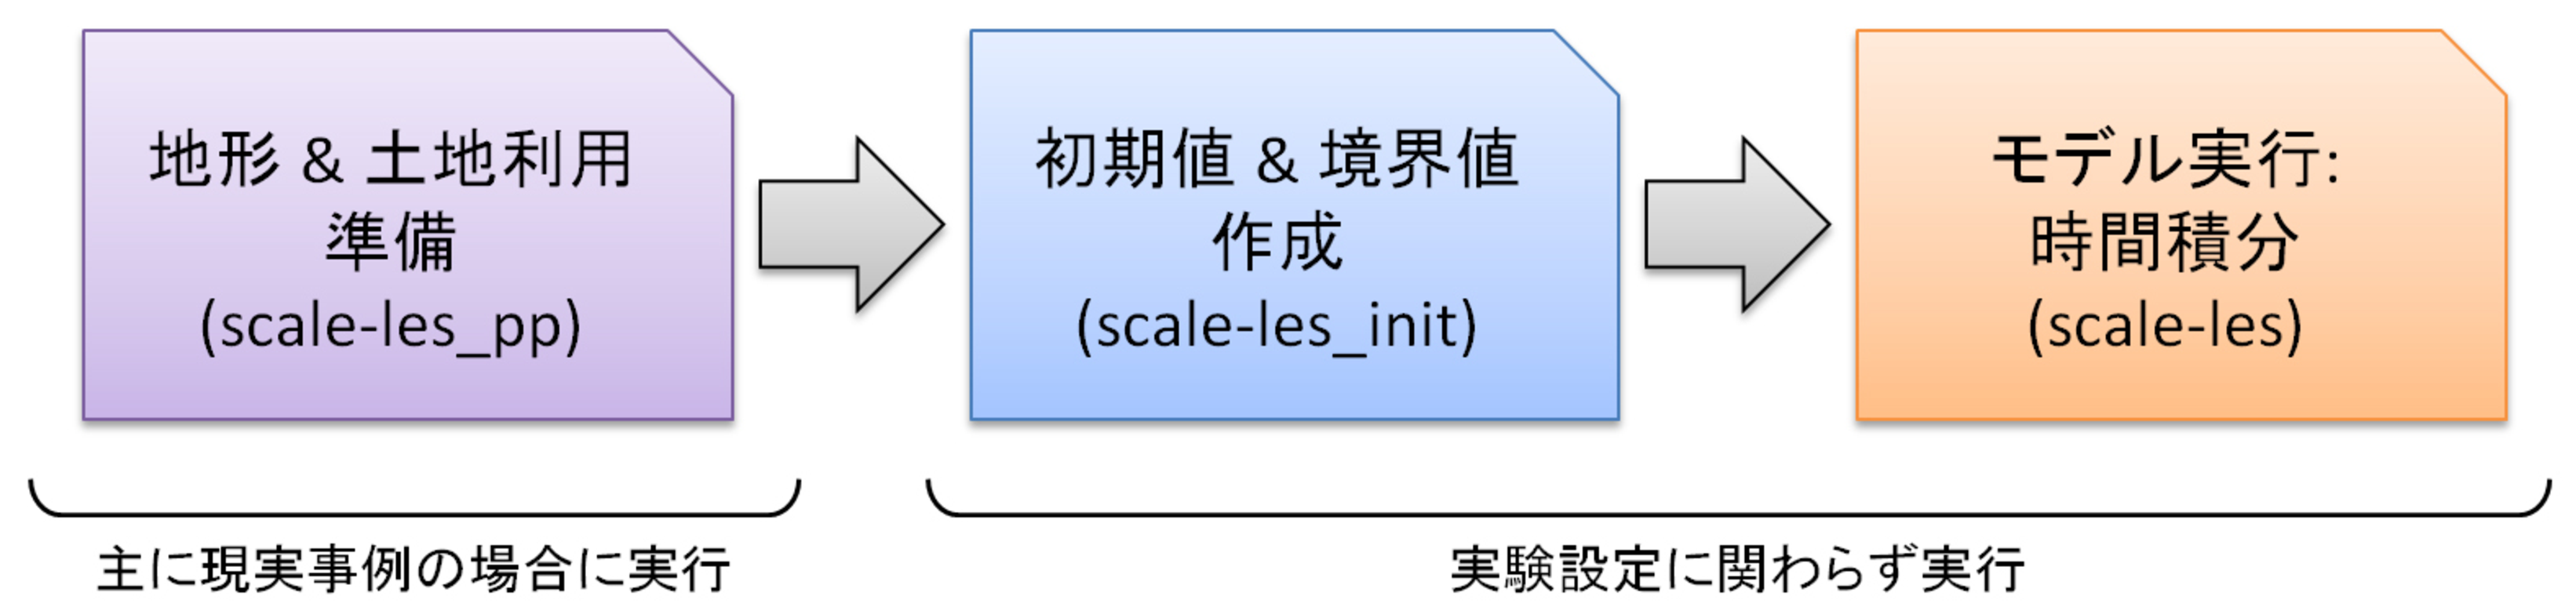
\includegraphics[width=0.9\hsize]{./figure/how_to_run.eps}\\
  \caption{SCALE-LESモデルの実行過程}
  \label{fig:howto}
\end{center}
\end{figure}


